\documentclass[xcolor=dvipsnames,4pt]{beamer}

\setbeamertemplate{navigation symbols}{}
\usefonttheme{professionalfonts}
\useinnertheme{circles}
\usepackage[spanish]{babel}
\usepackage[T1]{fontenc}
\usepackage[utf8]{inputenc}
\usepackage[orientation=portrait,size=custom,width=32,height=18]{beamerposter}

\usepackage[notocbib]{apacite}
\usepackage{multirow}
\usepackage{graphicx}
\usepackage{tikz}

\usecolortheme[named=Black]{structure}

\usetikzlibrary{arrows,shapes,positioning,backgrounds}

% My default font
%\usepackage{newcent}

% Computer Modern Bright font
%\usepackage{cmbright}

% Iwona light
\usepackage[light,math]{iwona}

% LX fonts
%\usepackage{lxfonts}

% Malvern
%\input T1fmv.fd
%\renewcommand*\sfdefault{fmv}
%\renewcommand*\familydefault{\sfdefault}

% Comfortaa
%\usepackage[default]{comfortaa}

%\setbeamercolor{frametitle}{fg=NavyBlue}
%\setbeamercolor{structure}{fg=NavyBlue}
%\setbeamercolor{normal text}{fg=black}
\setbeamercolor{alerted text}{fg=NavyBlue}
%\setbeamercolor{example text}{fg=red}

\newcommand{\cl}[1]{\multicolumn{1}{c}{#1}}

\newenvironment{changemargin}[2]{%
  \begin{list}{}{%
    \setlength{\topsep}{0pt}%
    \setlength{\leftmargin}{#1}%
    \setlength{\rightmargin}{#2}%
    \setlength{\listparindent}{\parindent}%
    \setlength{\itemindent}{\parindent}%
    \setlength{\parsep}{\parskip}%
  }%
\item[]}{\end{list}}

\begin{document}
\tikzstyle{every picture}+=[remember picture]
\tikzstyle{na} = [baseline=-.5ex]

\begin{frame}
\title{Galaxias Tempranas}
%\subtitle{}
\author{Alfredo J. Mej\'ia$^{1,2}$}

\date{\today}

\institute{$^{1}$Posgrado de F\'isica Fundamental\\ Universidad de Los Andes \and $^{2}$Centro de%
Investigaciones de Astronom\'ia%
}

\maketitle
\end{frame}

\begin{frame}{¿Qué son galaxias tempranas?}
\begin{changemargin}{-1cm}{-3cm}
\begin{columns}
\column{0.6\textwidth}
De la clasificación morfológica original de Hubble, se llama Galaxia Temprana (ETG en inglés) a aquellas que no poseen brazos espirales y que tienen una apariencia elíptica o circular en imágenes astronómicas.
\column{0.4\textwidth}
\begin{figure}
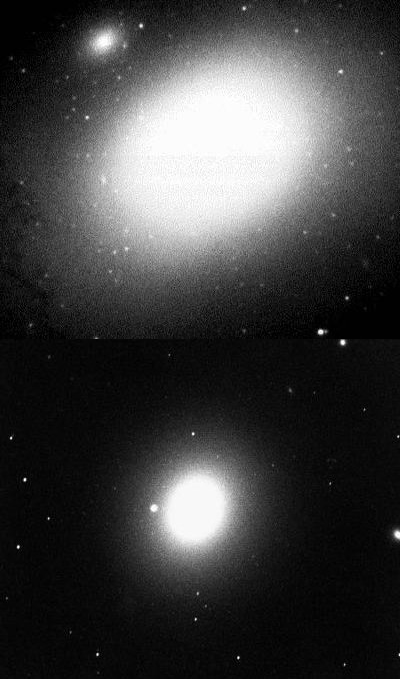
\includegraphics[scale=0.65]{img/m86anon_m49noao.png}
\end{figure}
\end{columns}
\end{changemargin}
\end{frame}


\begin{frame}{Clasificación morfológica de Hubble}
\begin{changemargin}{-1cm}{-1cm}
\begin{figure}
\centering
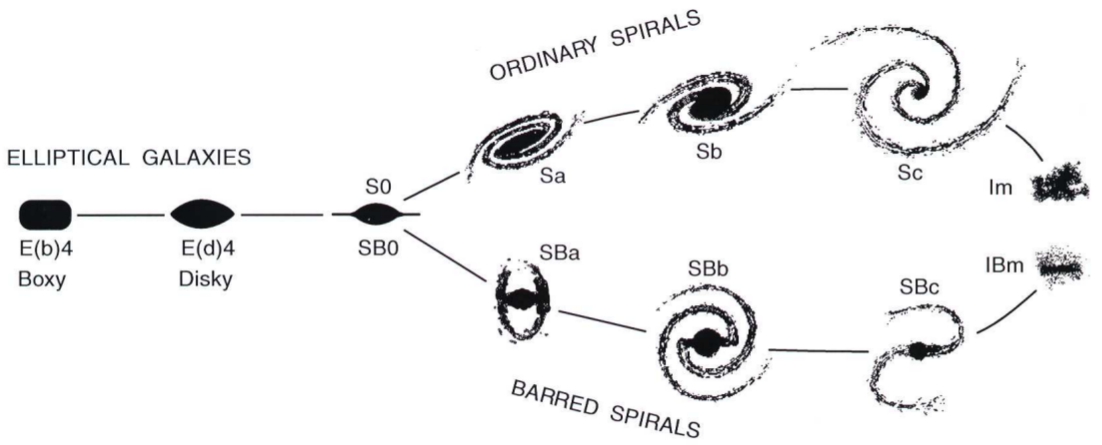
\includegraphics[scale=0.8]{img/hubble_diap.png}
\end{figure}
\end{changemargin}
\end{frame}

\begin{frame}{Perfil de brillo}
\begin{changemargin}{-1cm}{-1cm}
\begin{columns}
\column{0.5\textwidth}
\small
$$
\Sigma(R) = \Sigma_b\left(\frac{R_b}{R}\right)^\gamma\left[\frac{1}{2}-\frac{1}{2}\left(\frac{R}{R_b}\right)^\alpha\right]^{(\gamma-\beta)/\alpha}
$$
\bigskip
\bigskip
\bigskip
\begin{description}
\item[${\color{teal}R_b:}$] es el radio de corte.
\item[${\color{teal}\Sigma_b:}$] es el brillo superficial en $R_b$.
\item[${\color{teal}\alpha:}$] es la suavidad del corte.
\item[${\color{teal}\beta:}$] la pendiente asintótica para $R<R_b$.
\item[${\color{teal}\gamma:}$] la pendiente asintótica para $R>R_b$.
\end{description}
\column{0.5\textwidth}
\begin{figure}
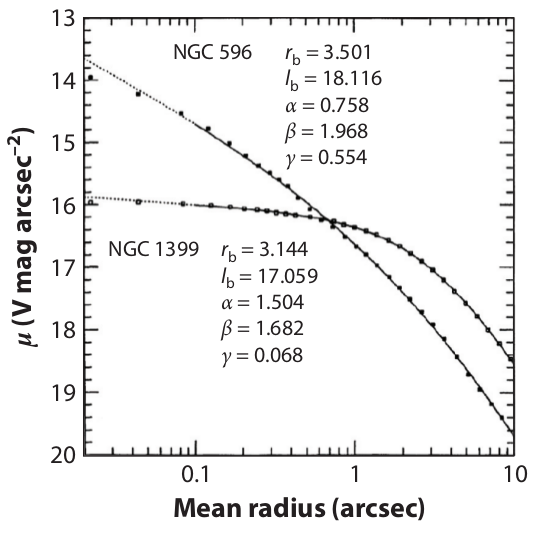
\includegraphics[scale=0.74]{img/perfil_brillo.png}
\end{figure}
\end{columns}
\end{changemargin}
\end{frame}

\begin{frame}{Fotometría vs. cinemática}
\begin{figure}
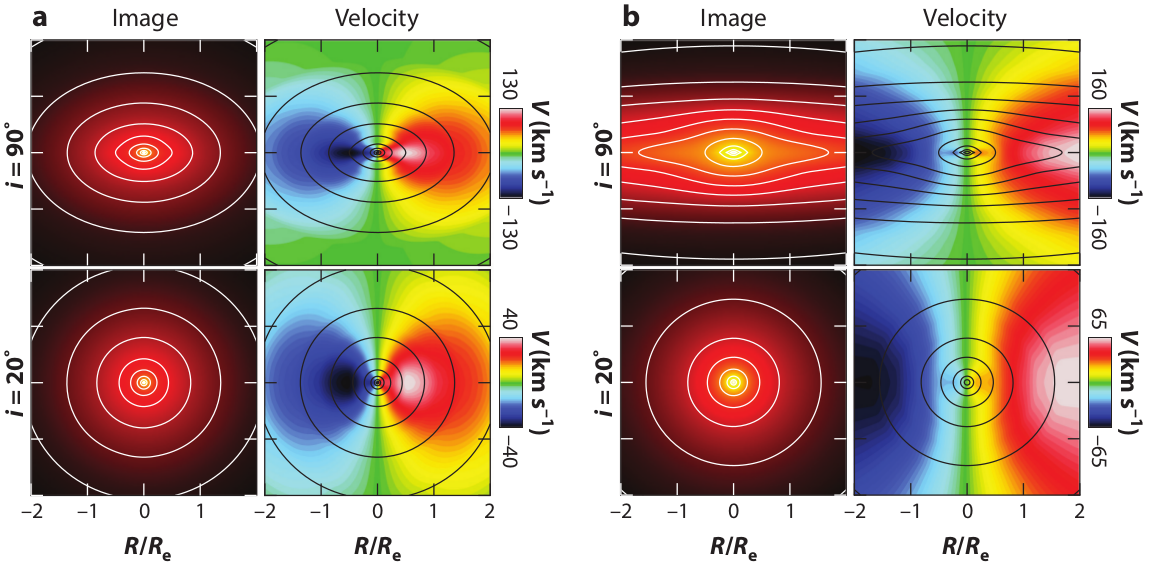
\includegraphics[scale=0.74]{img/isof_cin.png}
\end{figure}
\end{frame}

\begin{frame}{Fotometría vs. cinemática}
\begin{changemargin}{-1cm}{-1cm}
\begin{columns}
\column{0.5\textwidth}
{\bf Fotometría}
\bigskip
\bigskip
\bigskip
\begin{itemize}
\item Perfil de brillo.
\item Clasificación visual.
\item Contenido estelar.
\end{itemize}
\column{0.5\textwidth}
{\bf Cinemática}
\bigskip
\bigskip
\bigskip
\begin{itemize}
\item Perfil de velocidad.
\item Clasificación estructural.
\item Función de distribución.
\end{itemize}
\end{columns}
\end{changemargin}
\end{frame}

\begin{frame}{Contenido estelar de las ETGs}
\begin{changemargin}{-1cm}{-1cm}
\begin{columns}
\column{0.4\textwidth}
\small
La \emph{sobre-abundancia} de elementos $\alpha$ es un claro indicador de formación en una escala de tiempo corta, $\sim1$ Gaño.
\column{0.6\textwidth}
\begin{figure}
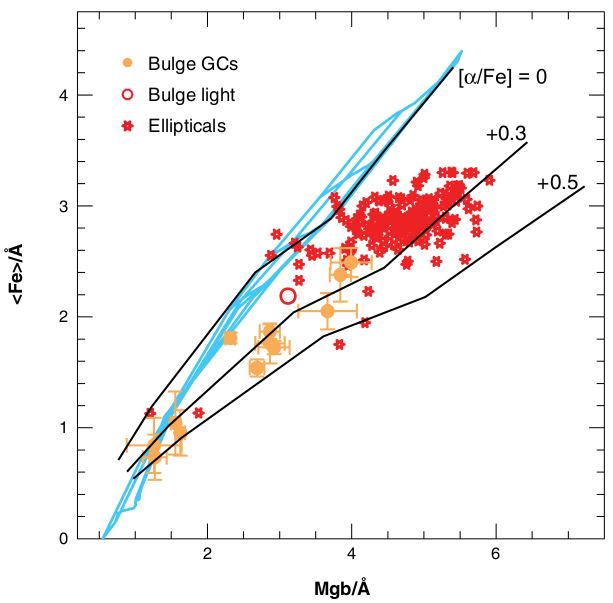
\includegraphics[scale=0.73]{img/alfa_enhance.png}
\end{figure}
\end{columns}
\end{changemargin}
\end{frame}

\begin{frame}{Contenido estelar de las ETGs}
\begin{changemargin}{-1cm}{-1cm}
\begin{columns}
\column{0.7\textwidth}
\begin{figure}
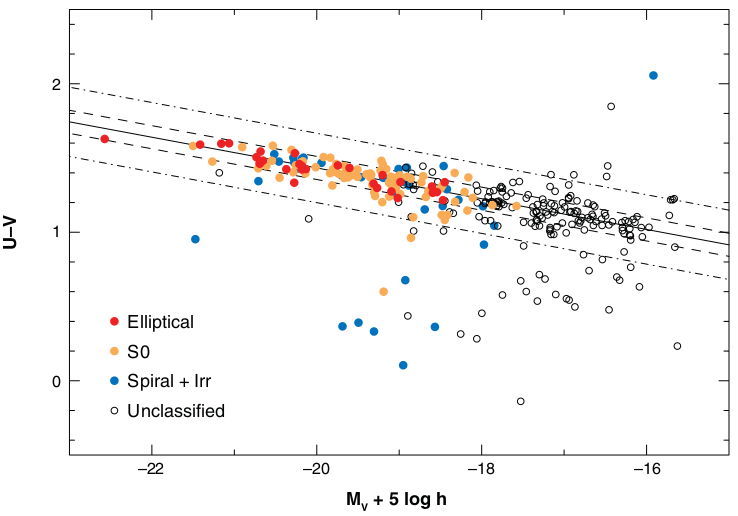
\includegraphics[scale=0.8]{img/cmd.png}
\end{figure}
\column{0.3\textwidth}
\small
Las ETGs forman una secuencia en el diagrama color-magnitud, llamada \emph{secuencia roja}.

El color $U-V$ no deja ver distinción entre la población estelar en las galaxias S0 y las Elípticas.
\end{columns}
\end{changemargin}
\end{frame}

\begin{frame}{Contenido estelar de las ETGs}
\begin{changemargin}{-1cm}{-1cm}
\begin{figure}
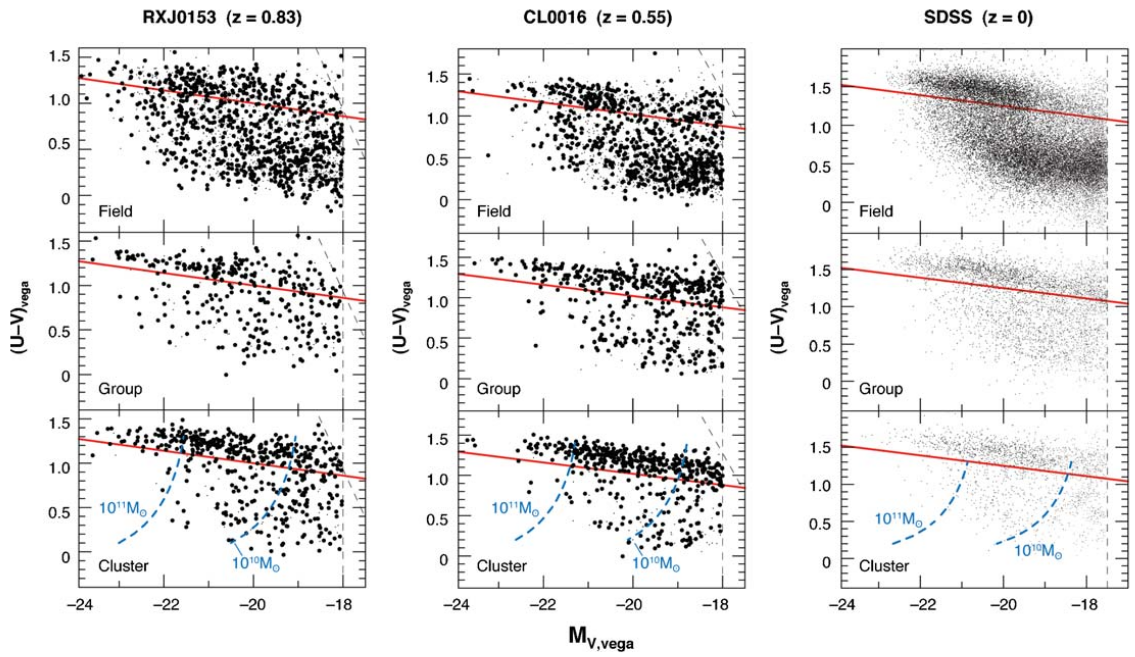
\includegraphics[scale=0.68]{img/cmd_z.png}
\end{figure}
\end{changemargin}
\end{frame}

\begin{frame}{Contenido estelar de las ETGs}
\begin{changemargin}{-1cm}{-1cm}
\begin{columns}
\column{0.5\textwidth}
\begin{figure}
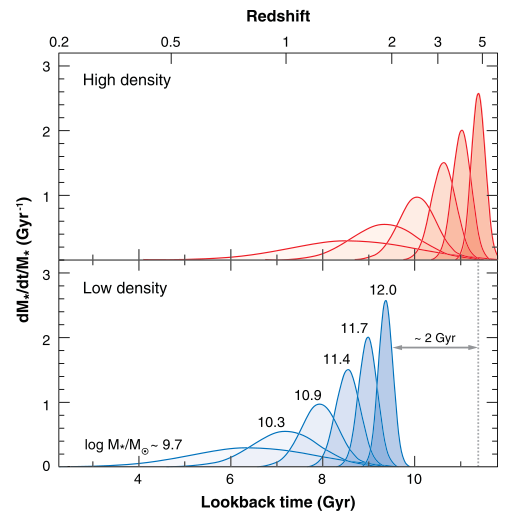
\includegraphics[scale=0.81]{img/sfhs.png}
\end{figure}
\column{0.5\textwidth}
\small
\begin{description}
\item[{\it\color{teal}Formación rápida.}] La sobre-abundancia $\alpha$ determina la escala temporal de formación de ETGs, i.e., el ancho de la tasa de formación estelar.
\item[{\it\color{teal}Evolución pasiva.}] La independencia de la secuencia roja con $z$ hasta $z\sim1$, sugiere que estas galaxias ya estaban ensambladas cuando el universo tenía la mitad de su edad actual.
\end{description}\end{columns}
\end{changemargin}
\end{frame}

\begin{frame}{Contenido estelar de las ETGs}
\begin{block}{Resumen}
\begin{itemize}
\item El estudio de las poblaciones estelares en ETGs no permite una separación clara entre las S0 y las E.
\item El hecho de que hasta $z\sim1$ la evolución haya sido pasiva dificulta los diagnósticos que podemos hacer usando información fósil.
\item Las observaciones de galaxias $z>2$ sufren del sesgo del progenitor y a $z>3$ están limitadas por nuestra tecnología actual.
\end{itemize}
\end{block}
\end{frame}

\begin{frame}{Cinemática y estructura de las ETGs}
\begin{block}{El modelado de la dinámica permite\ldots}
\begin{itemize}
\item \emph{virtualmente} obtener la distribución orbital,
\item reconstruir la estructura de la galaxia, y
\item obtener la distribución de masa \emph{total}.
\end{itemize}
\end{block}

\begin{block}{Sin embargo\ldots}
\begin{itemize}
\item son necesarios datos cinemáticos de muy buena calidad y
\item existen degeneraciones.
\end{itemize}
\end{block}
\end{frame}

\begin{frame}{Dicotomía cinemática}
\begin{changemargin}{-1cm}{-1cm}
\begin{figure}
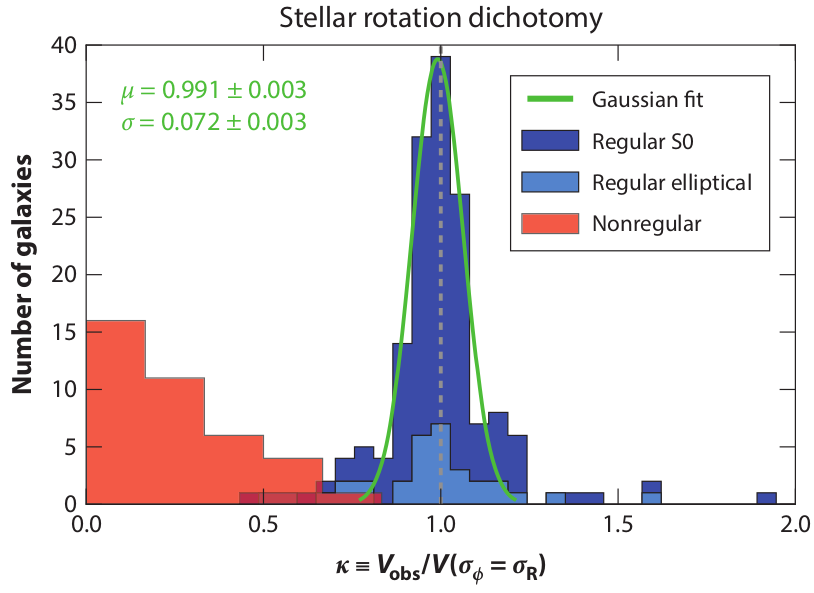
\includegraphics[scale=0.75]{img/dicotomia.png}
\end{figure}
\end{changemargin}
\end{frame}

\begin{frame}{Cinemática y estructura de las ETGs}
\begin{changemargin}{-1cm}{-1cm}
\begin{figure}
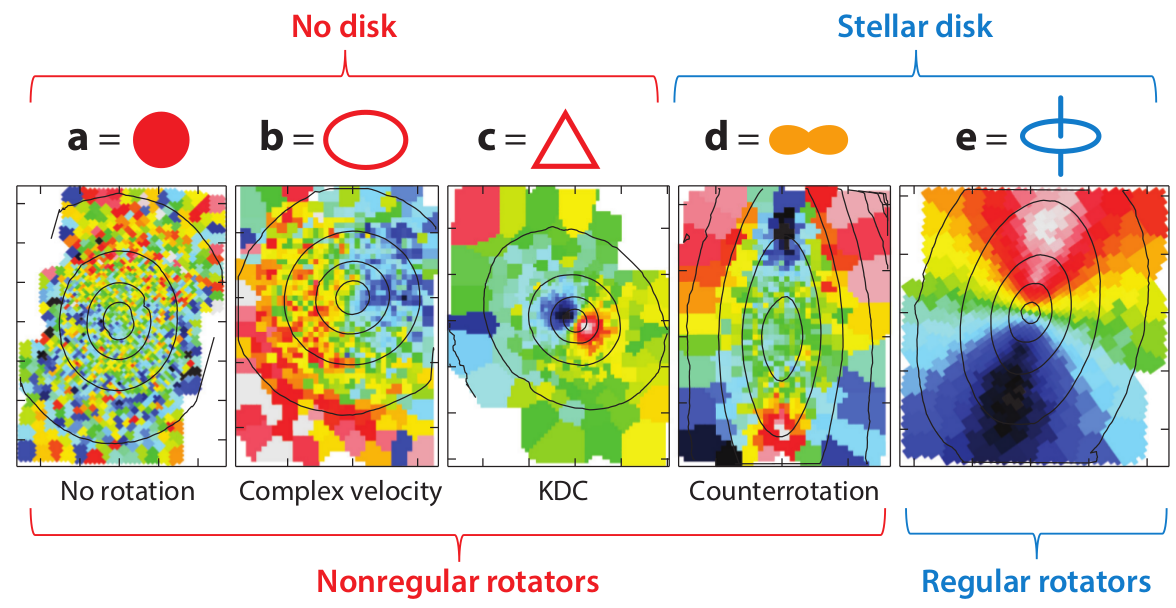
\includegraphics[scale=0.70]{img/cin_clas.png}
\end{figure}
\end{changemargin}
\end{frame}

\begin{frame}{El Plano Fundamental}
El teorema del virial implica que
$$
M\left<v^2\right> + W = 0,
$$
luego
$$
\left<v^2\right> = \frac{|W|}{M},
$$
que se puede reescribir como
$$
\sigma^2 \approx \frac{GM}{R_e} \approx \frac{G\Upsilon_e L}{2R_e} = \pi G\Upsilon_e I R_e.
$$
En escala logarítmica queda
$$
\log{R_e} = 2\log{\sigma} + 0.4\left<\mu\right> - \log{\Upsilon_e} + {\rm cons}.
$$
\end{frame}

\begin{frame}{El Plano Fundamental}
\begin{changemargin}{-1cm}{-1cm}
\begin{columns}
\column{0.4\textwidth}
\begin{figure}
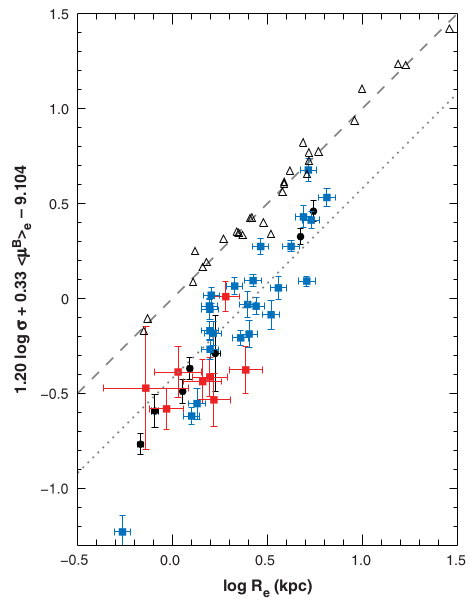
\includegraphics[scale=0.7]{img/fp.png}
\end{figure}
\column{0.6\textwidth}
La versión empírica del PF es
$$
\log{R_e} = 1.20\log{\sigma} + 0.33\left<\mu\right> + {\rm cons.}
$$
mientras que la versión teórica es
$$
\log{R_e} = 2\log{\sigma} + 0.4\left<\mu\right> - \log{\Upsilon_e} + {\rm cons}.
$$
\end{columns}
\end{changemargin}
\end{frame}

\begin{frame}{El Plano Fundamental}
\begin{block}{Resumen}
Ni las incertidumbres observacionales ni las suposiciones de fondo dan cuenta de la desviación del PF del equilibrio virial. Entre las fuentes más probables del origen de dicha desviación están:
\end{block}
\begin{itemize}
\item Variaciones en la contribución de materia oscura.
\item Variaciones en las poblaciones estelares.
\end{itemize}
\end{frame}

\begin{frame}{Relevancia de la materia oscura}
\begin{changemargin}{-1cm}{-1cm}
\begin{figure}
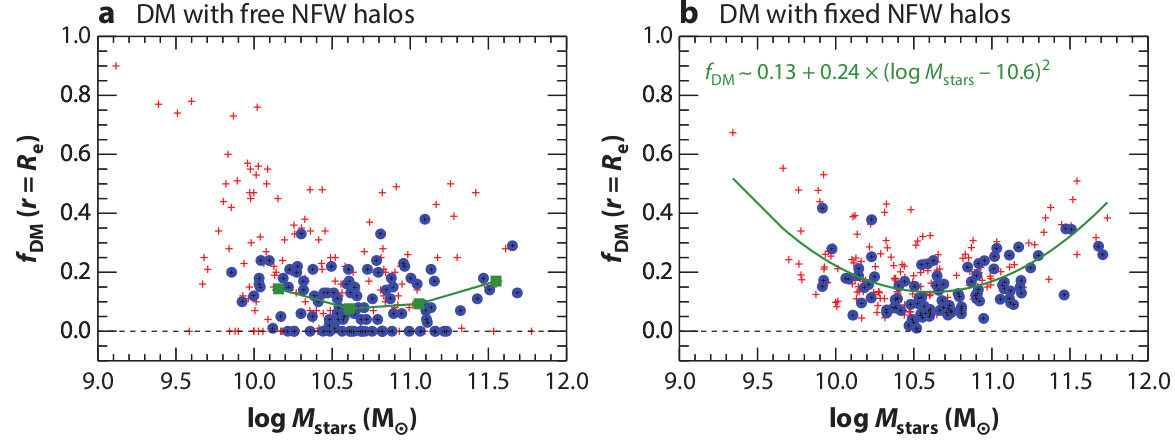
\includegraphics[scale=0.75]{img/mo_var.png}
\end{figure}
\end{changemargin}
\end{frame}

\begin{frame}{Variaciones poblacionales}
\begin{changemargin}{-1cm}{-1cm}
\begin{columns}
\column{0.7\textwidth}
\begin{figure}
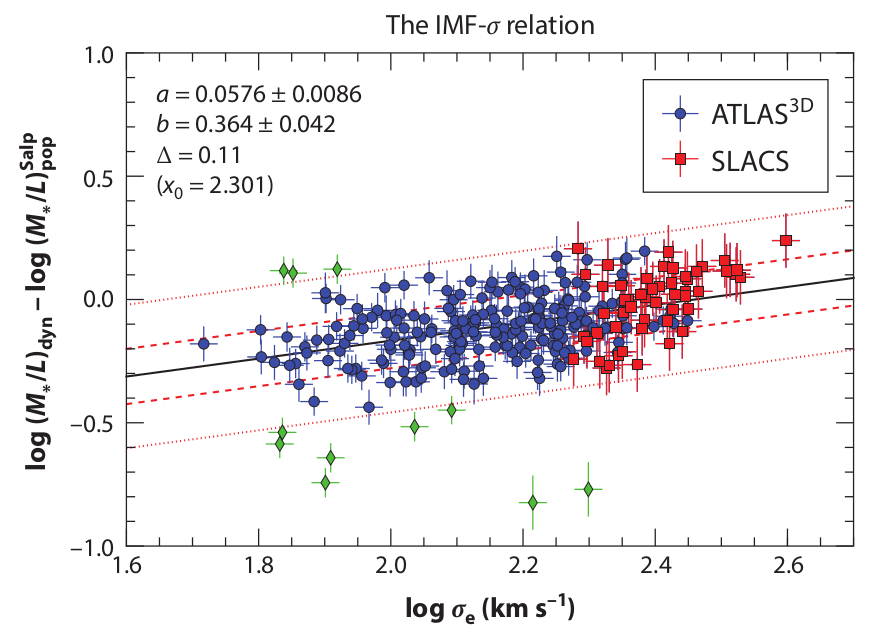
\includegraphics[scale=0.65]{img/imf_var.png}
\end{figure}
\column{0.3\textwidth}
\small
Las diferencias sistemáticas entre los resultados dinámicos y los poblacionales \emph{pueden interpretarse} como variaciones en la Función de Masa Inicial.
\end{columns}
\end{changemargin}
\end{frame}

\begin{frame}{Proyecciones del Plano de Masa}
\begin{changemargin}{-1cm}{-1cm}
\begin{figure}
\centering
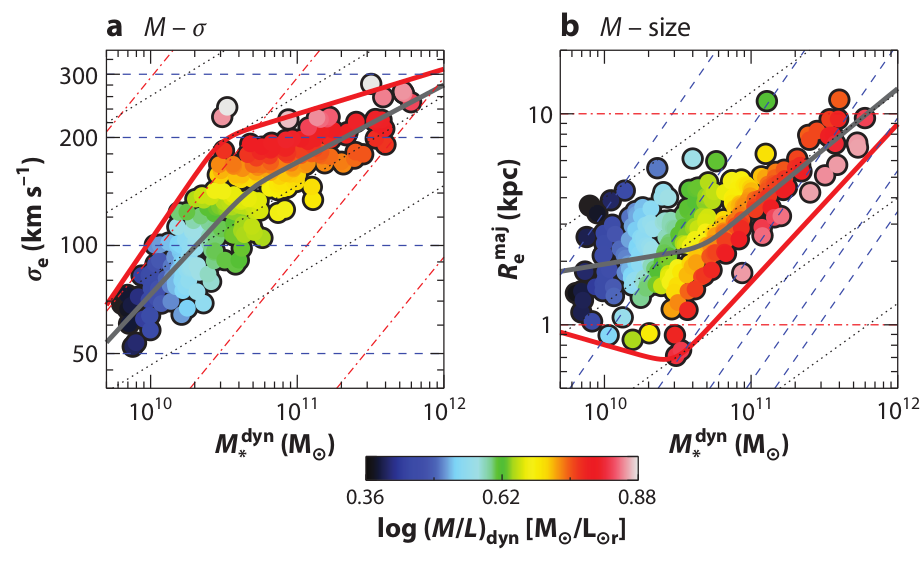
\includegraphics[scale=0.8]{img/r_m_pred.png}
\end{figure}
\end{changemargin}
\end{frame}

\begin{frame}{Proyección $R_e$--$M$}
\begin{changemargin}{-1cm}{-1cm}
\begin{figure}
\centering
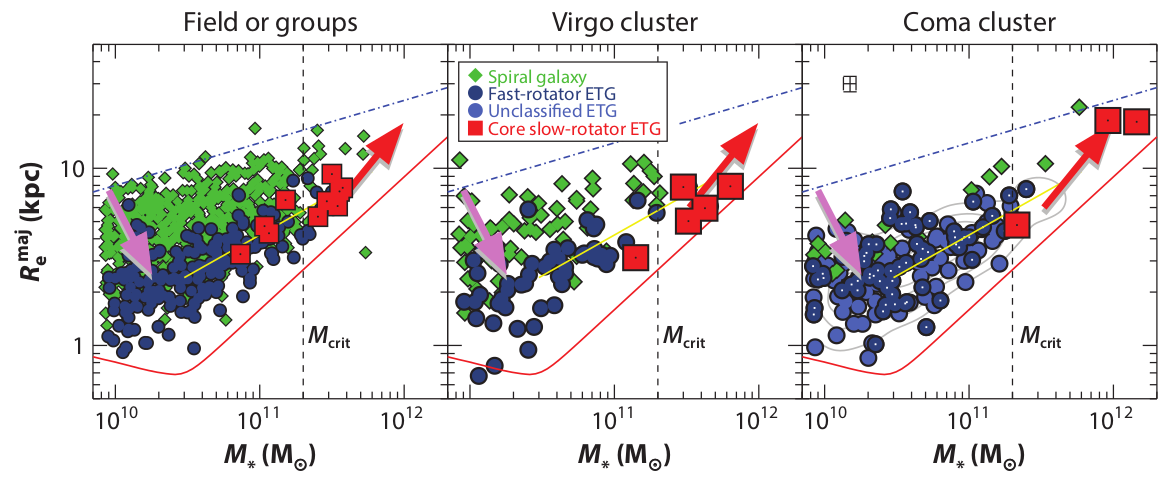
\includegraphics[scale=0.75]{img/r_m_clusters.png}
\end{figure}
\end{changemargin}
\end{frame}

\begin{frame}{Proyección $R_e$--$M$}
\begin{changemargin}{-1cm}{-1cm}
\begin{figure}
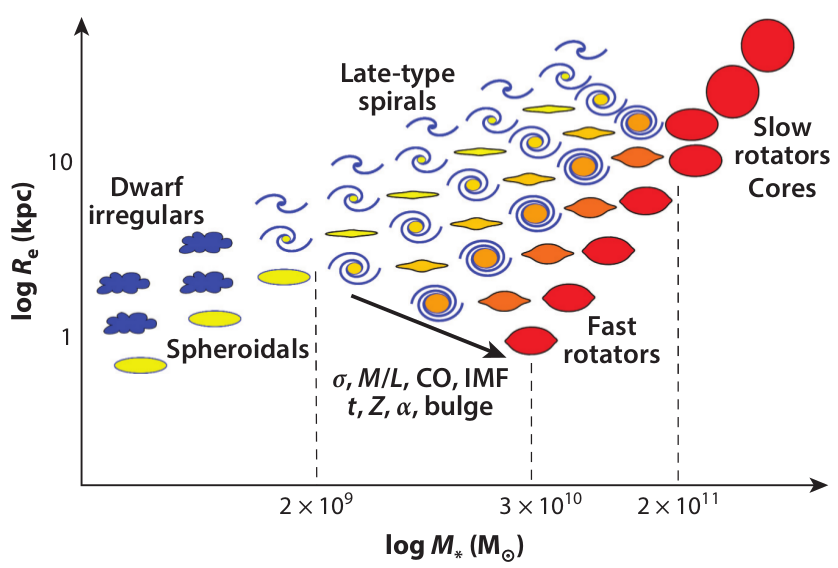
\includegraphics[scale=0.75]{img/r_m_esquema.png}
\end{figure}
\end{changemargin}
\end{frame}

\begin{frame}{Proyección $R_e$--$M$}
\begin{changemargin}{-1cm}{-1cm}
\begin{figure}
\centering
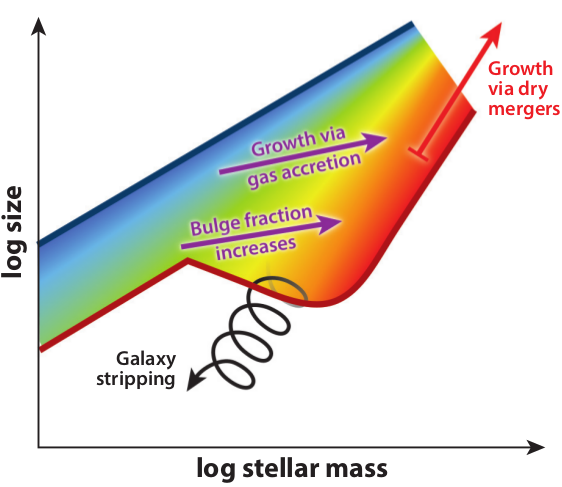
\includegraphics[scale=0.8]{img/size_mass_esquema.png}
\end{figure}
\end{changemargin}
\end{frame}

\begin{frame}{Morfología físicamente motivada}
\begin{changemargin}{-1cm}{-1cm}
\begin{figure}
\centering
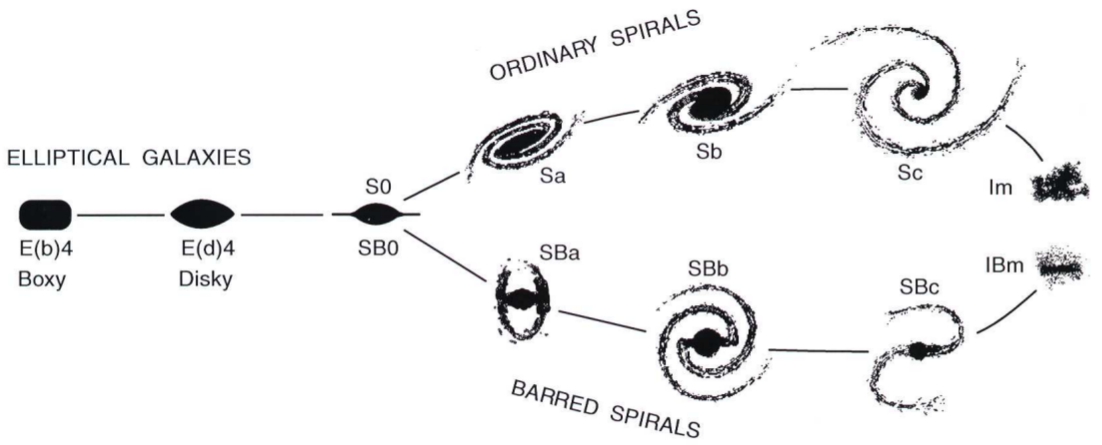
\includegraphics[scale=0.8]{img/hubble_diap.png}
\end{figure}
\end{changemargin}
\end{frame}

\begin{frame}{Morfología físicamente motivada}
\begin{changemargin}{-1cm}{-1cm}
\begin{figure}
\centering
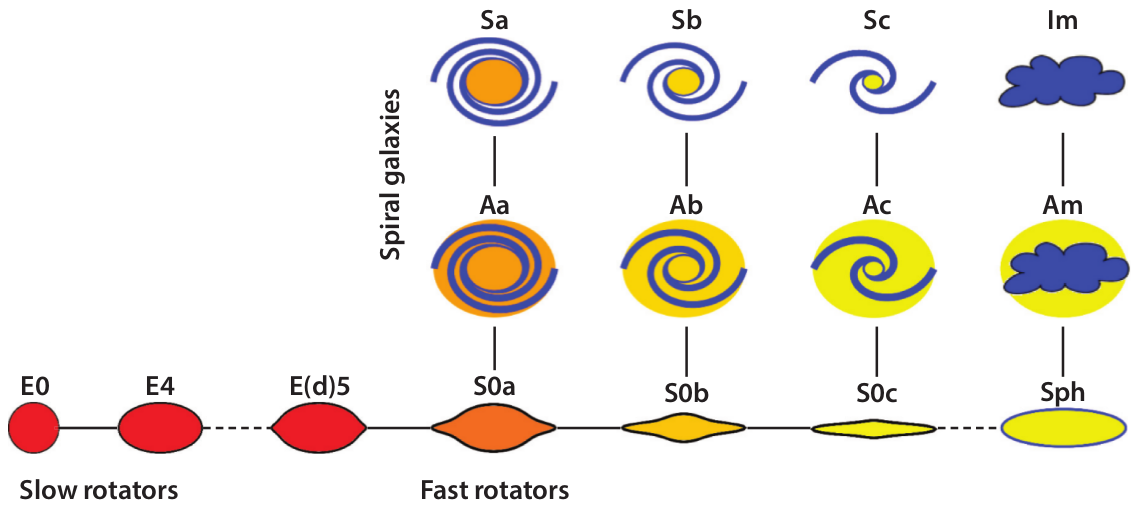
\includegraphics[scale=0.8]{img/comb.png}
\end{figure}
\end{changemargin}
\end{frame}

\begin{frame}{Resumen}
\begin{itemize}
\item Los estudios de poblaciones estelares han permitido inferir que las galaxias tempranas que vemos hoy ya se habían formado para $z\sim1$.
\item La evidencia fósil en la espectroscopía ha puesto en manifiesto la existencia de una sobre-abundancia de elementos $\alpha$.
\item Los dos puntos anteriores nos permiten inferir que las galaxias tempranas se han formado en una escala de tiempo muy corta.
\item Es claro también que existe una dependencia de dicha escala y de la masa (y edad) estelar con el ambiente: \alert{las galaxias en ambientes más densos se ensamblan más rápido y adquieren masas mayores}.
\end{itemize}
\end{frame}

\begin{frame}{Resumen}
\begin{itemize}
\item La información cinemática permite una separación de las galaxias tempranas en dos subclases: \alert{soportadas por rotación y soportadas por dispersión de velocidades}.
\item Ya que estos sistemas no están dinámicamente relajados, implica que han tenido canales de formación distintos.
\item Una forma natural de combinar los estudios poblacionales y los de dinámica es ofrecida por las relaciones de escala, en este caso el Plano Fundamental.
\item Aunque la interpretación física del Plano Fundamental aún está en debate, todo parece indicar que su desviación de la predicción teórica está relacionada con variaciones de las poblaciones estelares.
\item El Plano de Masa se ajusta a la interpretación del equilibrio virial y su interpretación ha permitido construir una visión detallada de la evolución de las galaxias tempranas y de sus posibles canales de formación.
\end{itemize}
\end{frame}

\begin{frame}{Cinemática y estructura}
\begin{changemargin}{-1cm}{-1cm}
\begin{figure}
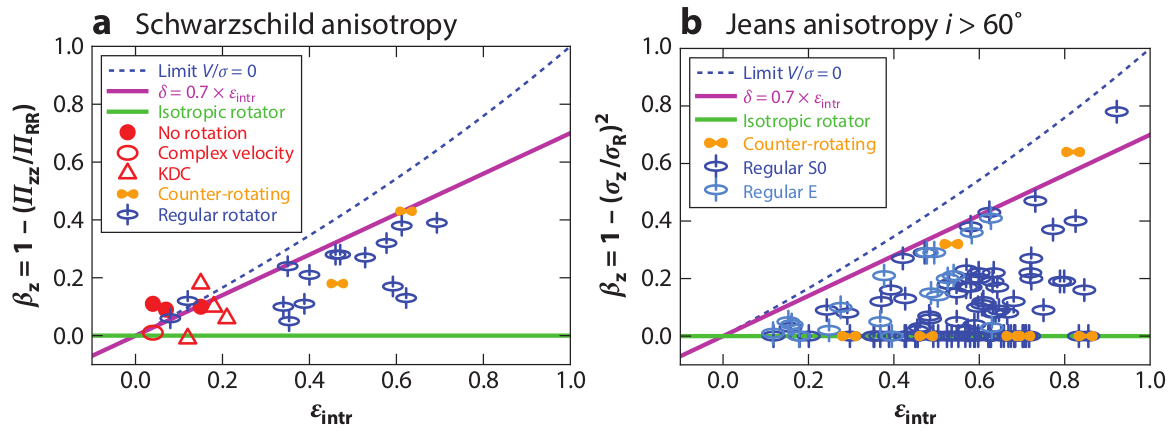
\includegraphics[scale=0.67]{img/dinamic.png}
\end{figure}

\begin{columns}
\small
\column{0.5\textwidth}
$$
\epsilon_{\rm int} = 1 - \sqrt{1+\epsilon(\epsilon-2)/\sen^2{i}}.
$$
\column{0.5\textwidth}
\begin{description}
\item[{\color{teal}$\epsilon_{\rm int}:$}] elipticidad intrínseca.
\item[{\color{teal}$\epsilon:$}] elipticidad observada.
\item[{\color{teal}$i:$}] ángulo de inclinación ($90^{\rm o}$ de canto).
\end{description}
\end{columns}
\end{changemargin}

\end{frame}

\begin{frame}{Cinemática y estructura}
\begin{changemargin}{-1cm}{-1cm}
\begin{block}{}
\begin{figure}
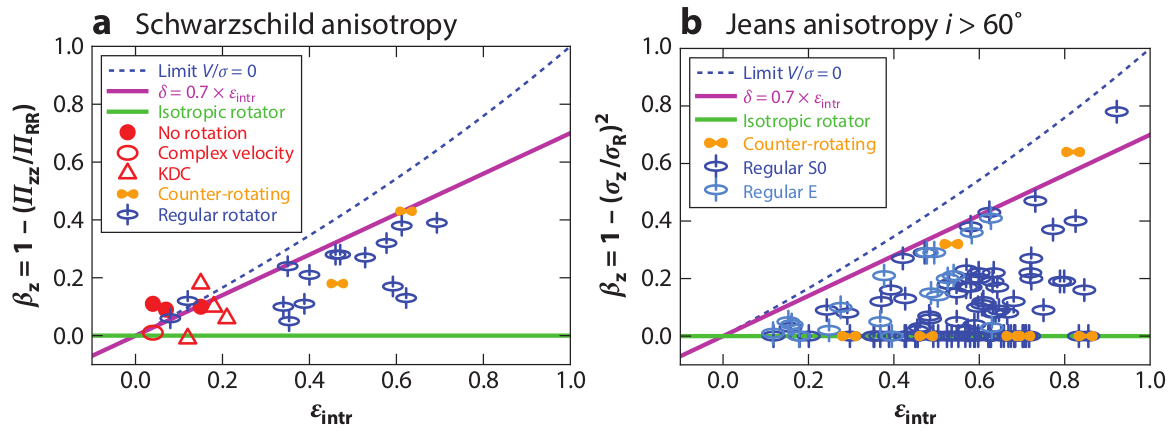
\includegraphics[scale=0.67]{img/dinamic.png}
\end{figure}
\end{block}

\begin{columns}
\small
\column{0.5\textwidth}
$$
\Pi_{kk} = \int \rho\sigma_k^2{\rm d}^3x.
$$
\column{0.5\textwidth}
\begin{description}
\item[{\color{teal}$\Pi_{kk}:$}] anisotropía en la dirección $k$.
\item[{\color{teal}$\rho:$}] densidad estelar.
\item[{\color{teal}$\sigma_k:$}] dispersión de velocidades.
\end{description}
\end{columns}
\end{changemargin}
\end{frame}

\begin{frame}{Proyección $R_e$--$M$ versus $z$}
\begin{changemargin}{-1cm}{-1cm}
\begin{figure}
\centering
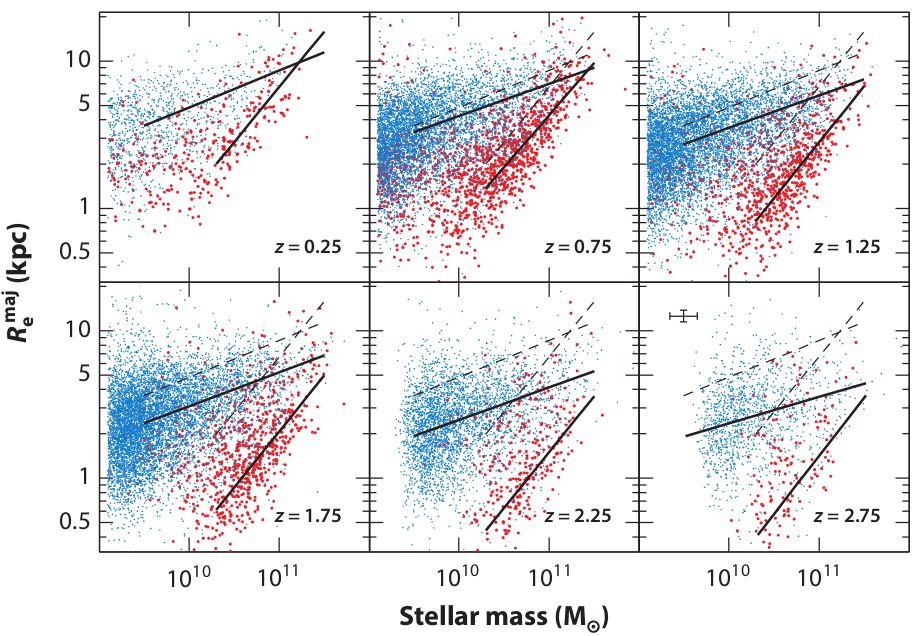
\includegraphics[scale=0.7]{img/r_m_z.png}
\end{figure}
\end{changemargin}

\end{frame}

\begin{frame}{Formación jerárquica}
\begin{changemargin}{-1cm}{-1cm}
\begin{figure}
\centering
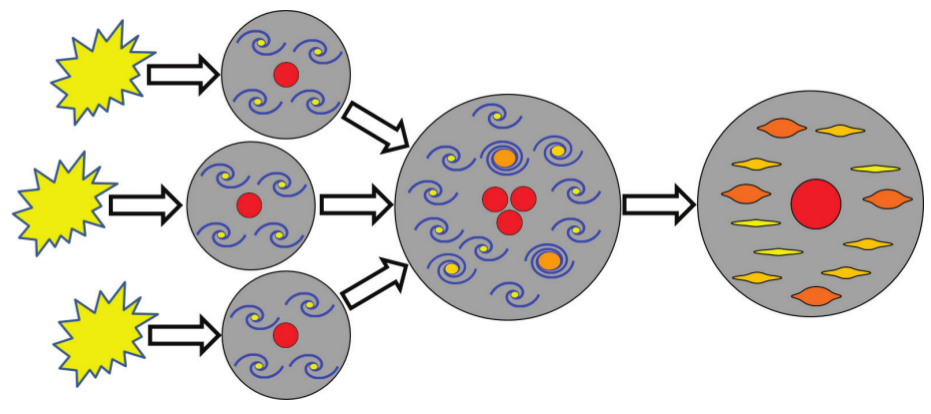
\includegraphics[scale=0.9]{img/jer.png}
\end{figure}
\end{changemargin}
\end{frame}

\begin{frame}{La función de masa de las galaxias a $z\sim0$}
\begin{changemargin}{-1cm}{-1cm}
\begin{columns}
\column{0.5\textwidth}
\begin{figure}
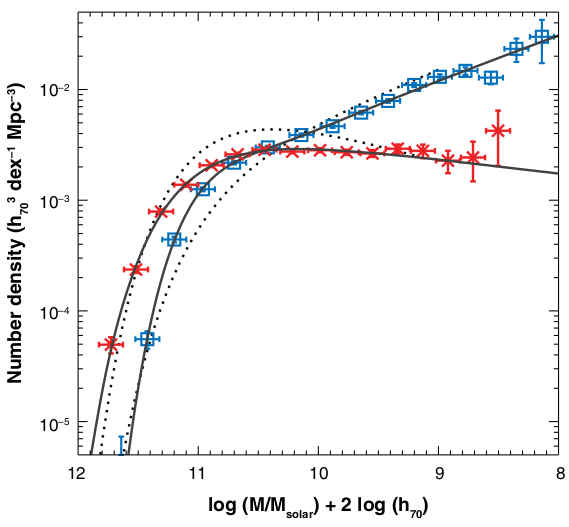
\includegraphics[scale=0.73]{img/mf.png}
\end{figure}
\column{0.5\textwidth}
\small
Distribución de masa de las {\color{teal}Galaxias Tardías} y de las {\color{red}Galaxias Tempranas}. Existen ETGs en casi todos los bines de masa, pero solo a $10^{11}$ M$_\odot$ el número de estas galaxias es más importante que el de las demás clases morfológicas.
\end{columns}
\end{changemargin}
\end{frame}

\end{document}
